\section{Durchführung}
\label{sec:Durchführung}
Der Pumpstand wird wie in Abbildung \ref{fig:Aufbau} aufgebaut. Dabei ist es wichtig möglichst genau 
zu arbeiten, damit keine Lecks druch falsch angebrachte Gummis und Flansches entstehen. Danach wird 
der Pumpstand mit der Drehschieberpumpe evakuiert. Stellt sich nach ca. 10 Minuten ein Druck 
zwischen 3 und \SI{5}{\hecto\pascal} ein, dann kann die Turbopumpe hinzugeschaltet werden. 
Dann wird der Rezipient ca. 15 Minuten mit einem Heißluftföhn erwärmt. Das 
führt dazu, dass Wasserablagerungen im Rezipienten ausdampfen und die Desorptionsrate 
abnimmt. Bei starker Wasseransammlung, kann ein Gasanfall beobachtet werden, sofern die 
Messgeräte eingeschaltet sind. Wird nun ein Enddruck zwischen \SI{2e-3}{} und \SI{8e-3}{\pascal} 
erreicht gilt der Aufbau als dicht und es kann mit der Messung angefangen werden.
\newline
Da der Enddruck des Aufbaus erreicht ist und die Turbopumpe schon arbeitet, bietet es sich an 
mit der Messung zur Turbopumpe anzufangen.  
\begin{SCfigure}
  \caption[justification=centering]{Foto des Versuchsaufbaus mit nummerierten Komponenten; \\
1. Rezipient\\
2. Dosierventiel\\
3,5. Kugelventiel \\
4. Glühkathodenvakuummeter\\
6. Turbomolekularpumpe\\
7. Pirani-Digitalvakuummeter\\
8. Pirani-Analogvakuummeter\\
9,11. Schlauch\\
10. Drehschieberpumpe\\
12. Kreuzstück, \\
an dem ein Rohr mit 7. und 8., \\
die Schläuche 9. und 11.\\
 und ein Kugelventil \\
 zur Turbopumpe befestigt ist.\\
13. Anzeigen von 4. und 8. \\
14. Steuergerät der Turbopumpe \\
}
  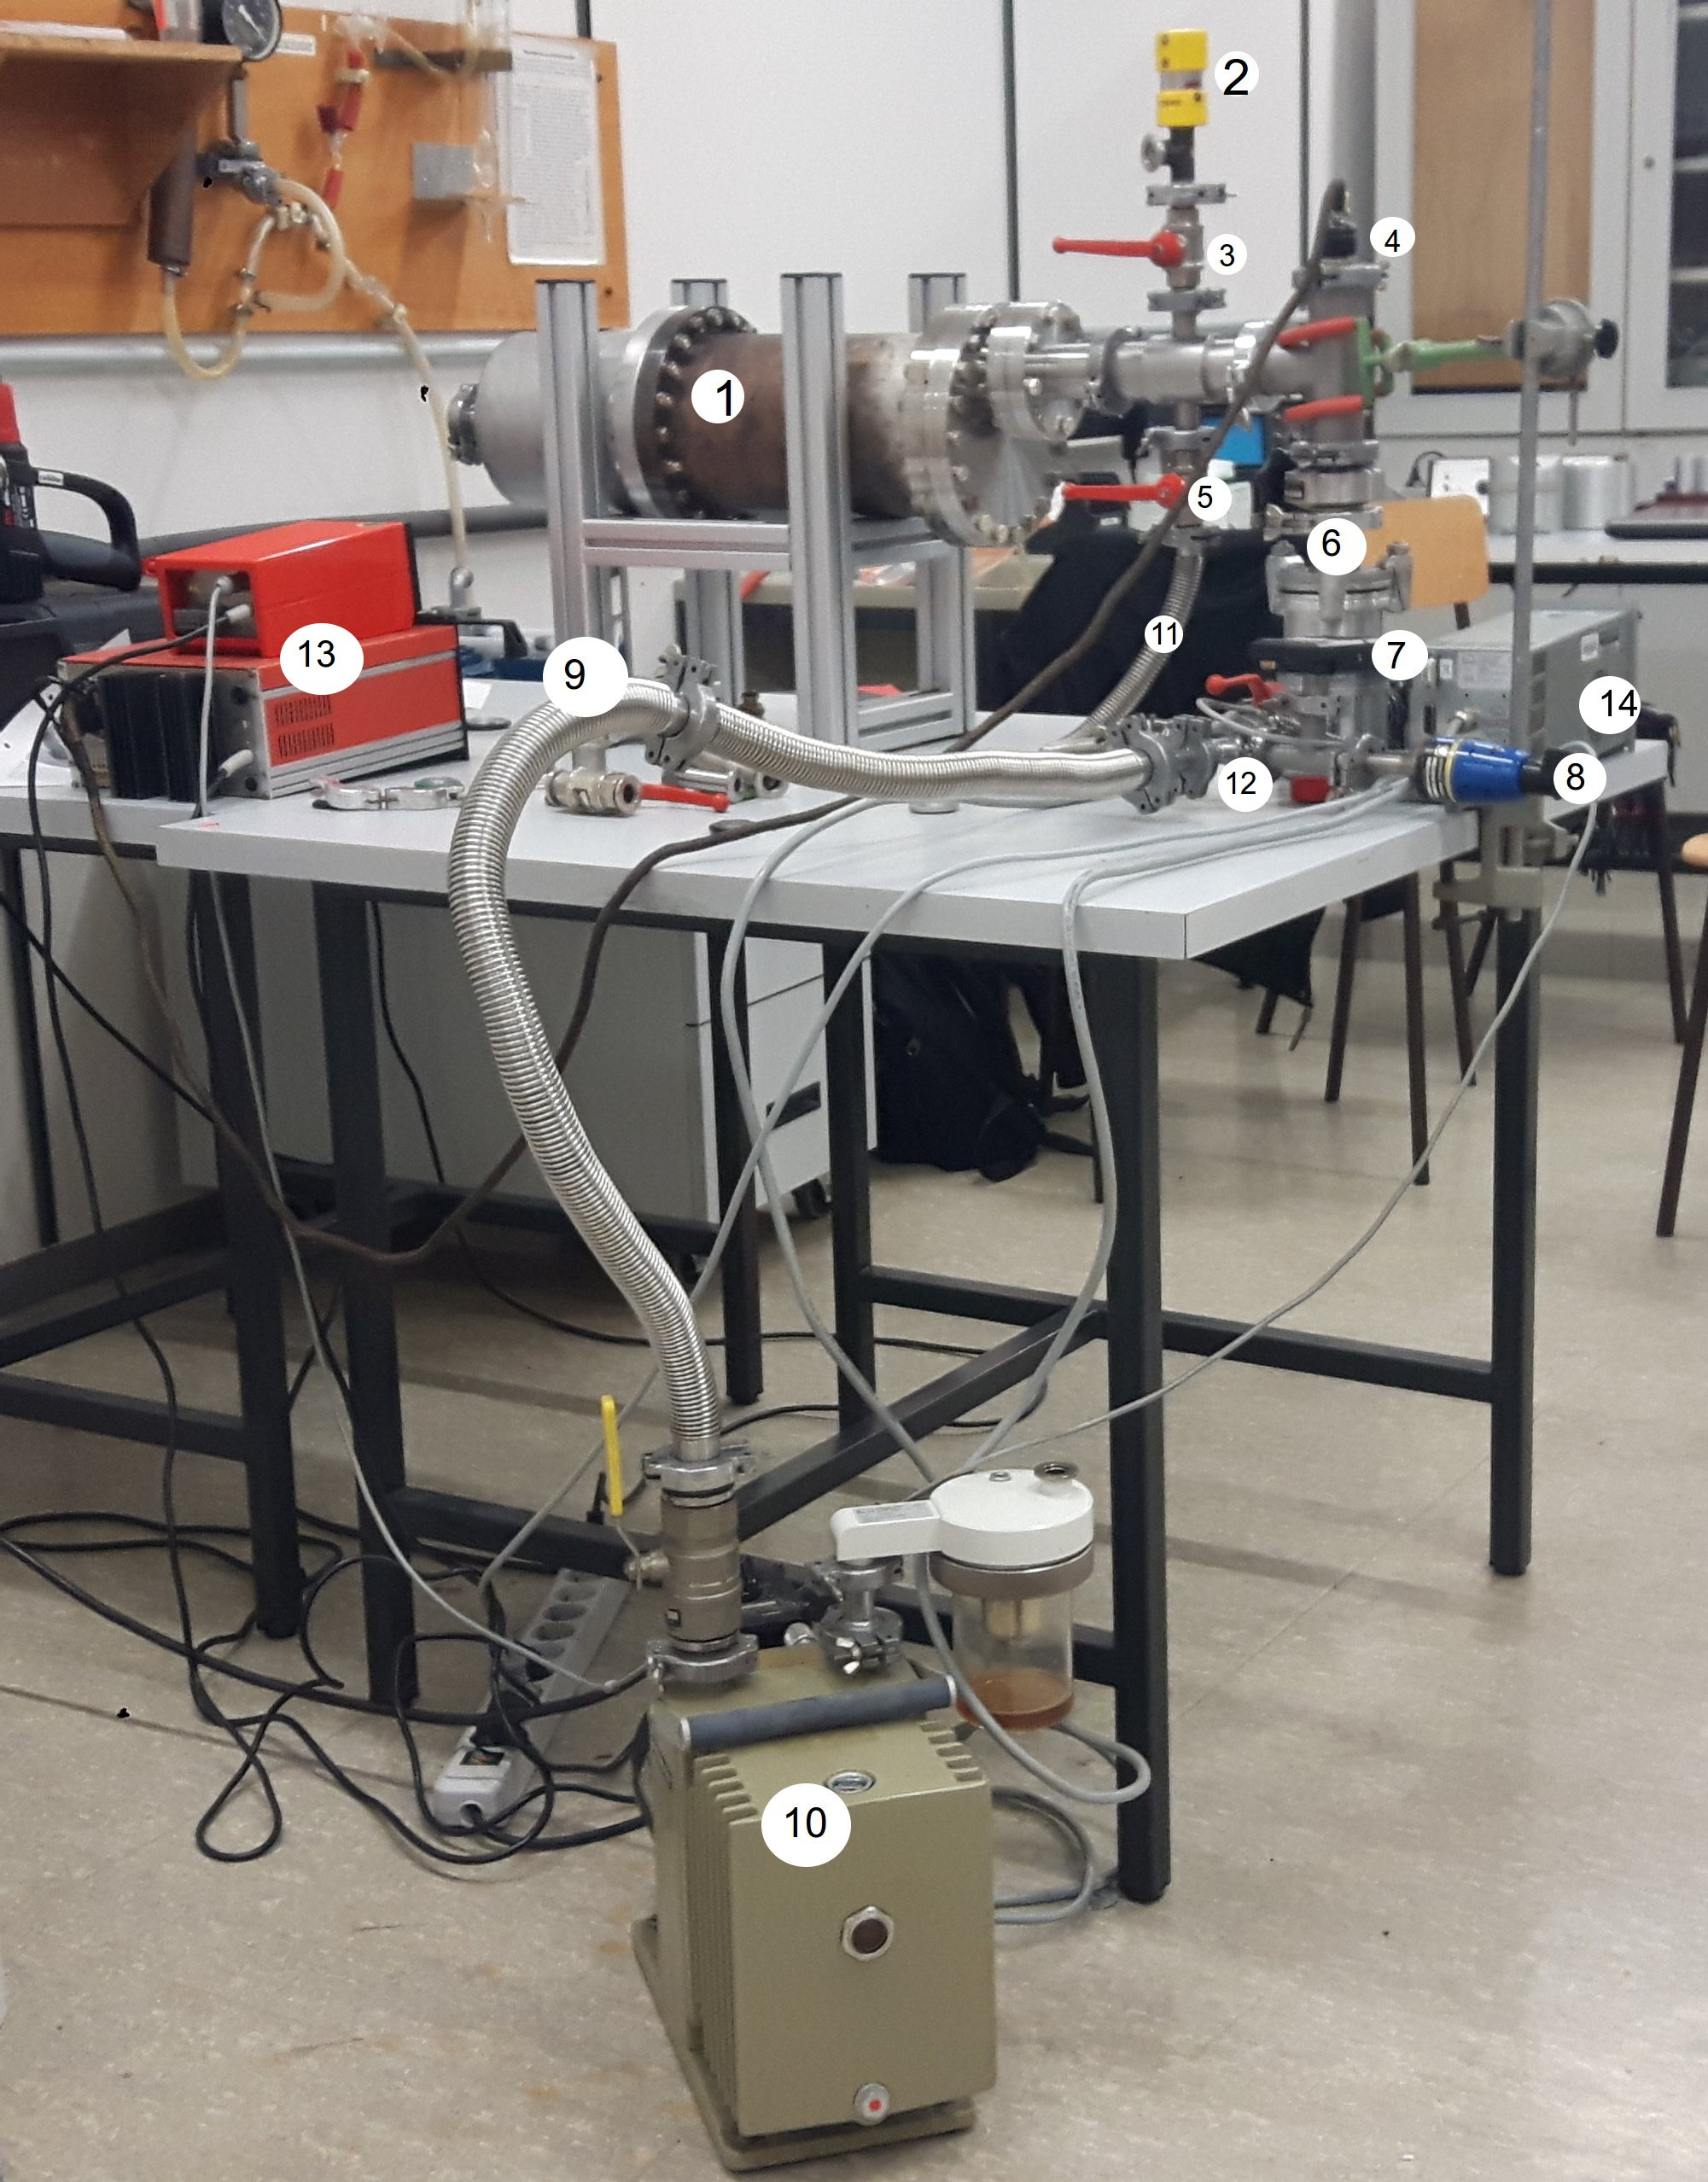
\includegraphics[height  = 10cm]{pics/V3B2.jpg}
  \label{fig:Aufbau}
\end{SCfigure}


